\subsection{Impact of lattice calculations of  $x$-space PDFs}
\label{sec:projectionsxspace}

Following the study of the impact of
lattice-QCD calculations of PDF moments,
in this section we perform an initial exploration of the
potential constraints that future lattice QCD calculations
of $x$-space PDFs can provide on the global analysis.
%
Specifically, we will focus on the isotriplet
combination $x u-x d$ (and $x\Delta u - x\Delta d$
in the polarized case), which is
perhaps the quark combination for which
more theoretical
progress has been achieved recently.

Following the same Bayesian reweighting procedure that
has been employed to quantify the impact of the
PDF moments in Sect.~\ref{sec:projections:rw},
we have generated pseudo-data for the isotriplet
combinations
\be
\label{eq:isotriplet_unpol}
u(x_i,Q^2)-d(x_i,Q^2) \, \quad{\rm and} \, \quad
\bar{u}(x_i,Q^2)-\bar{d}(x_i,Q^2) \, , \quad i=1,\ldots,N_x \, ,
\ee
for the unpolarized case, and for
\be
\label{eq:isotriplet_pol}
\Delta u(x_i,Q^2)-\Delta d(x_i,Q^2) \, \quad{\rm and} \, \quad
\Delta\bar{u}(x_i,Q^2)-\Delta\bar{d}(x_i,Q^2) \, , \quad i=1,\ldots,N_x \, ,
\ee
for the polarized case, with $N_x$ being the number of points
in $x$-space that are being sampled and we
take $Q^2=4$ GeV$^2$, consistently with the choice used
in the case of the PDF moments.

We consider here three scenarios, denoted by scenario D, E, and F,
for the total uncertainty $\delta_L$
that will be assigned to
the lattice-QCD calculations of the specific quark
combinations listed in Eqns.~(\ref{eq:isotriplet_unpol})
and~(\ref{eq:isotriplet_pol}).
%
First of all we indicate the values of $\left\{ x_i \right\}$
that have been chosen for this exercise.
%
With the motivation that the lattice-QCD computation is expected to have the
smallest systematic uncertainties at large $x$,
we have chosen the $N_x=5$ points to be
\be
x_i = 0.70\, ,0.75,\, 0.80,\, 0.85, \, 0.90 \, .
\ee
Then
for each scenario we assume that that the total error of the lattice calculation
is the same for each value of $\left\{ x_i \right\}$, and
moreover we neglect the possible correlations between neighboring $x$-points.
%
Specifically,
we have assumed  that we have $\delta_{L}=12\%, 6\%$ and 3\% for scenarios
D, E, and F, respectively.
%
Note also that we assume the same values of $\delta_{L}$ for the polarized
and unpolarized cases, as well as for both the quark
and the antiquark isotriplet combinations Eqns.~(\ref{eq:isotriplet_unpol})
and~(\ref{eq:isotriplet_pol}).

The results of this exercise are summarized
in Fig.~\ref{fig:impactxspace}, where we show the
ratio of PDF uncertainties to the original
  NNPDF3.1 (NNPDFpol1.1) in the fits where lattice-QCD pseudo-data
  on $x$-space PDFs has been added to the global unpolarized
  (polarized) analysis via reweighting.
  %
  Specifically, we show the impact on the PDF uncertainties
  in $\bar{u}$ and $\bar{d}$ at large-$x$ in the upper
  plots, with the corresponding comparison for $\Delta\bar{u}$
  and $\Delta\bar{d}$ in the lower plots.
  %
  From this comparison, we find that
  indeed these lattice-QCD calculations can reduce significantly
  the errors of the large-$x$ unpolarized and polarized
  antiquarks.
  %
  Taking into account that the PDF uncertainties on the large-$x$
  antiquarks to begin with are rather large, and that they
  enter a number of important BSM search channels
  (such as for instance for new heavy gauge bosons $W'$ and $Z'$)
  is clear that such calculations would have direct
  phenomenological implications.
  %
  Note that the in a Monte Carlo approach such as NNPDF, the
PDF uncertainties fluctuate themselves, specially at low-scales,
explaining the wiggles in these plots.

%-------------------------------------------------------------------
\begin{figure}[!t]
\centering
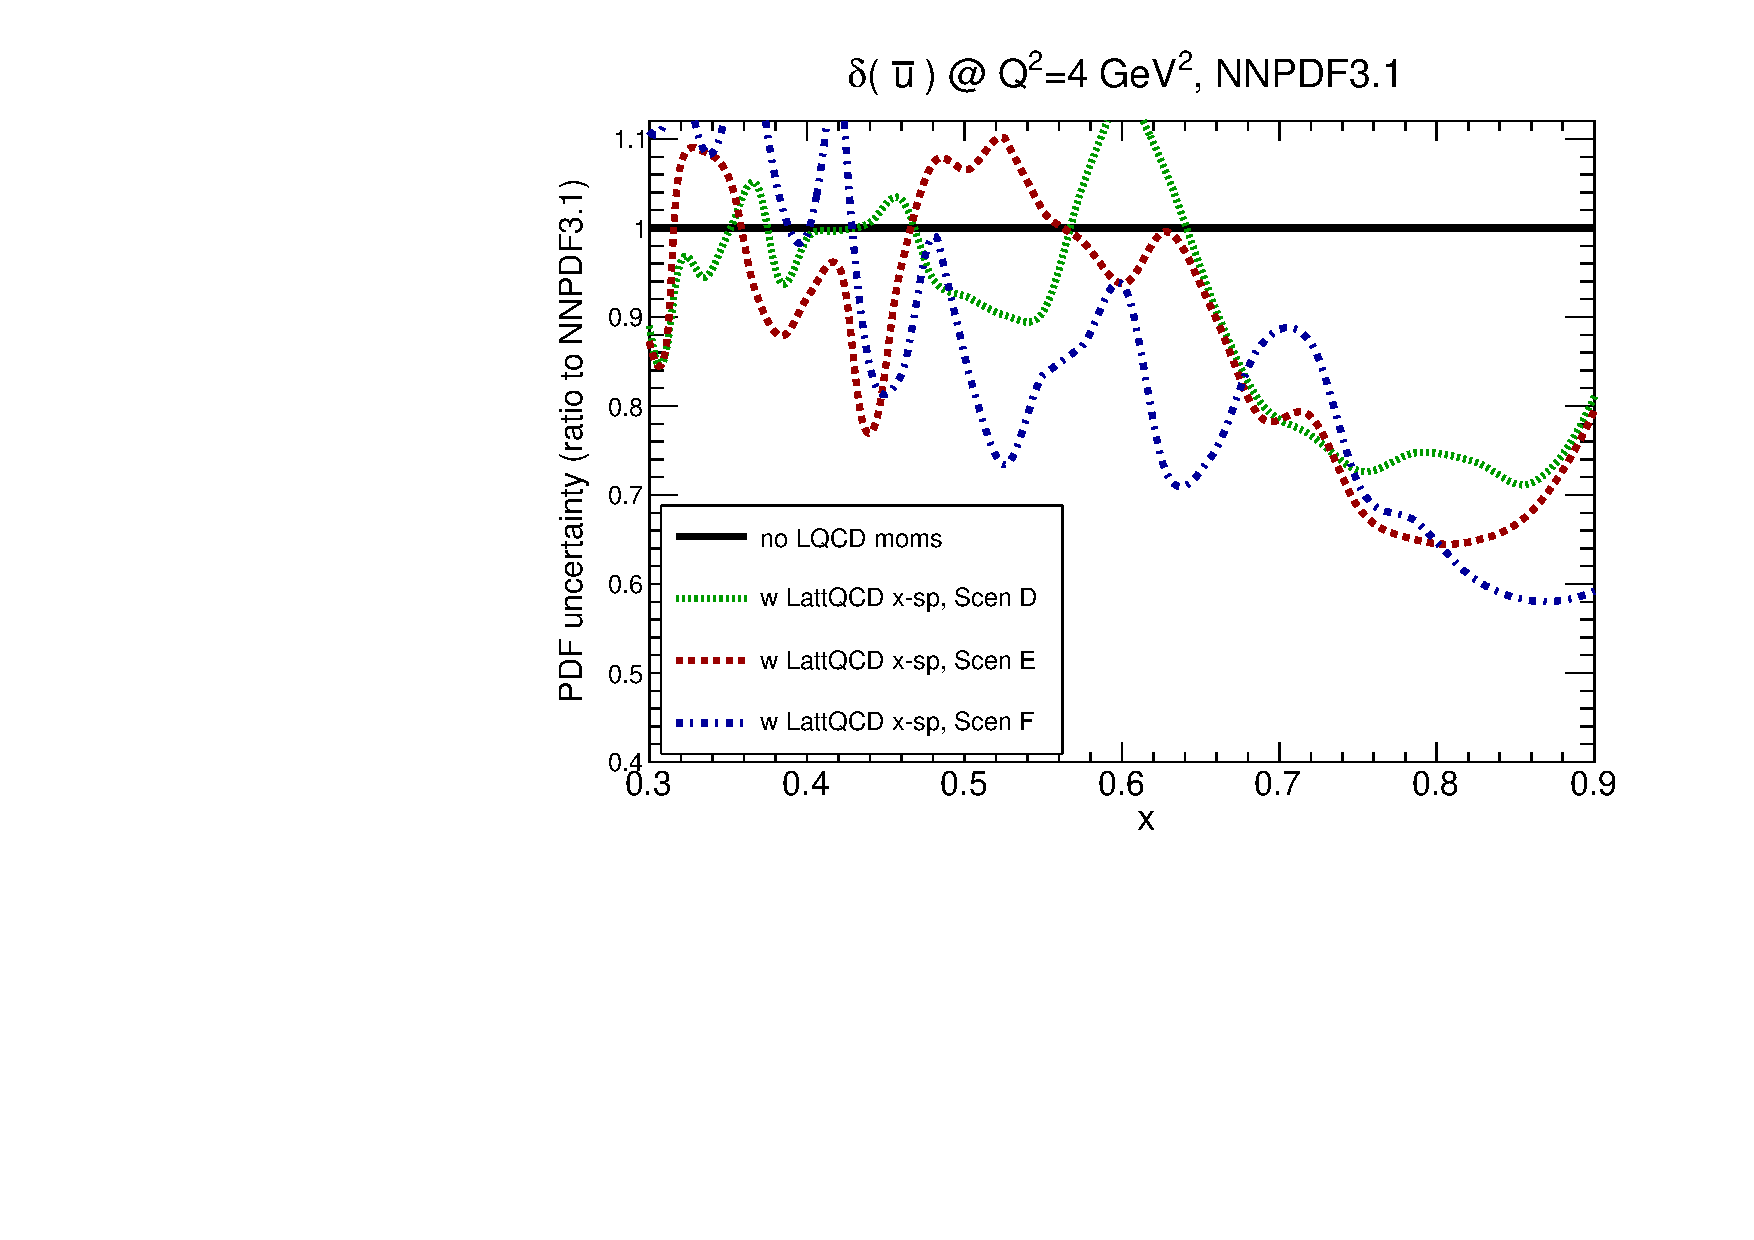
\includegraphics[scale=0.45]{plots/xubar-unpol-lattice-relerr-xdata-xspace.pdf}
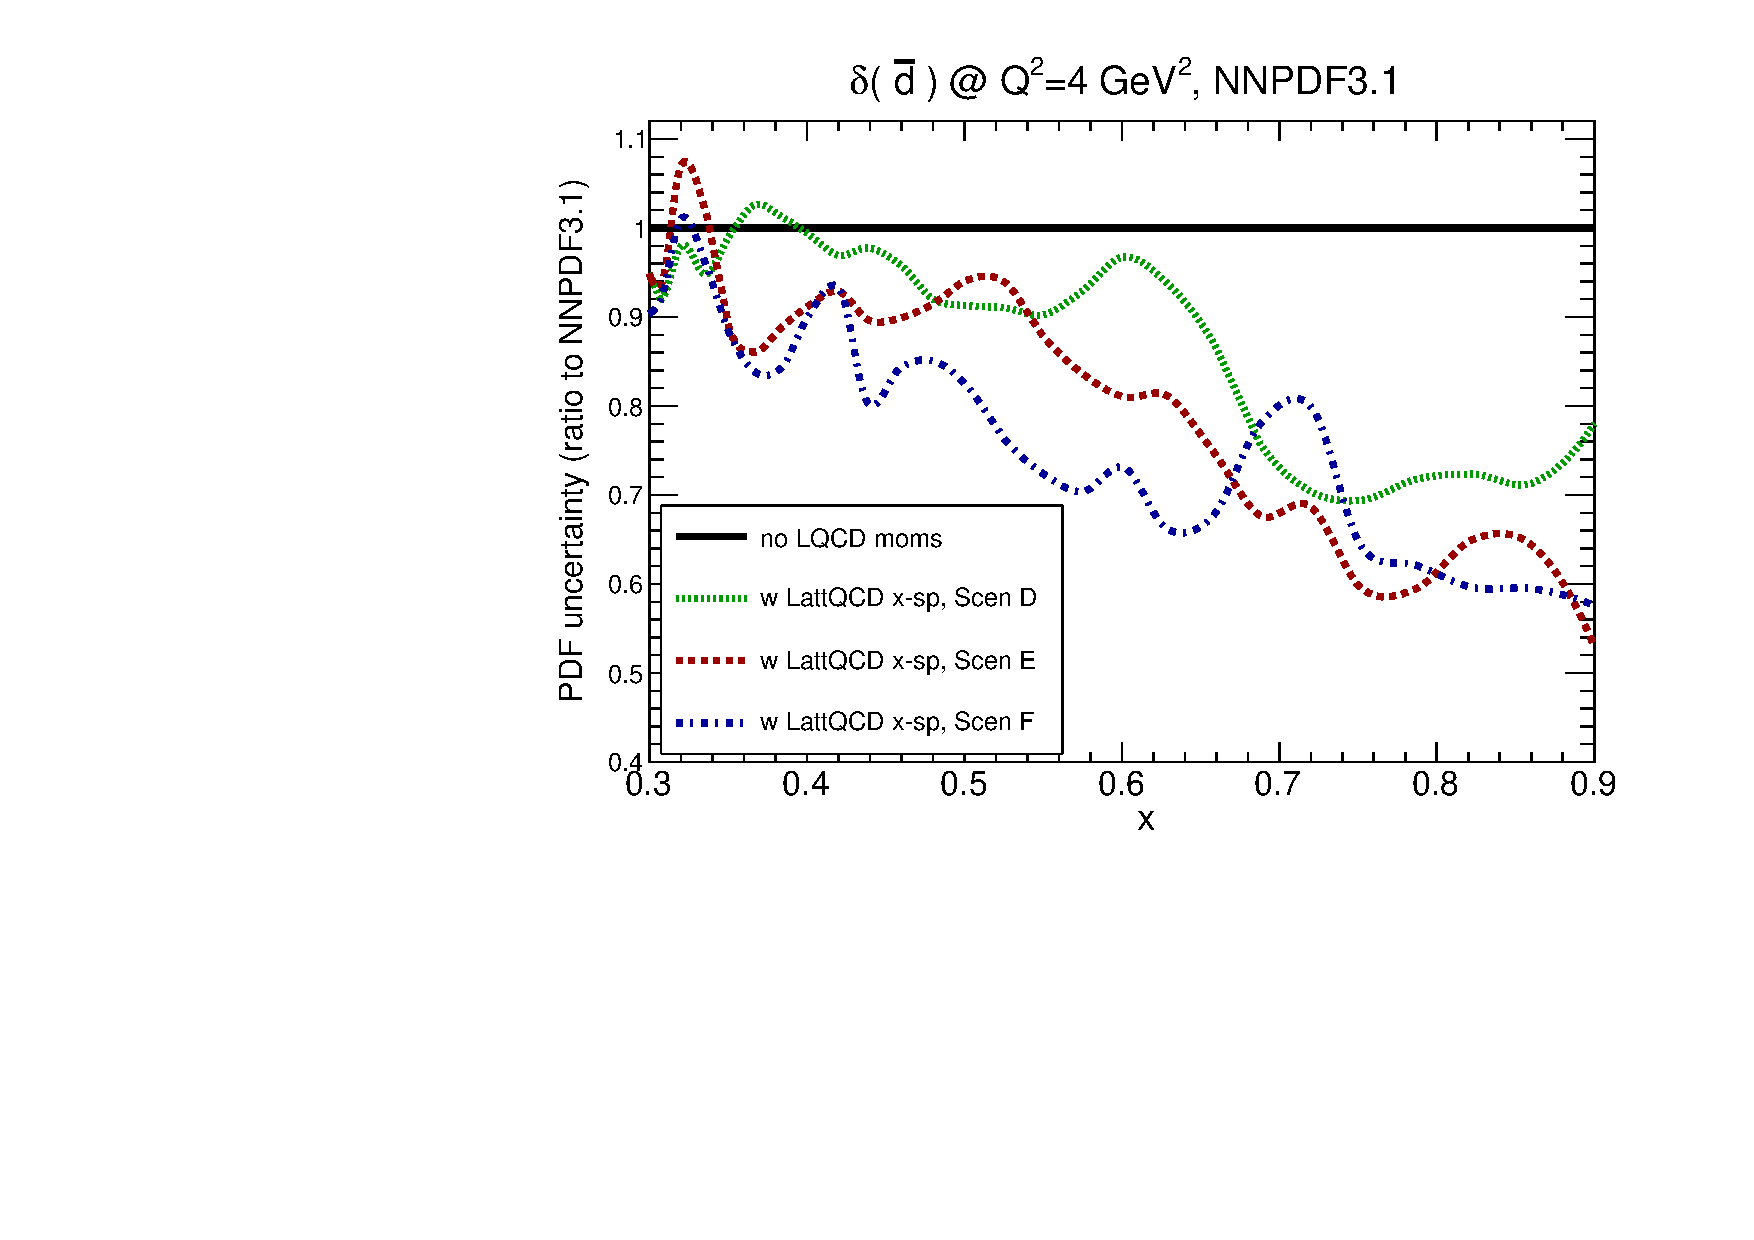
\includegraphics[scale=0.45]{plots/xdbar-unpol-lattice-relerr-xdata-xspace.pdf}
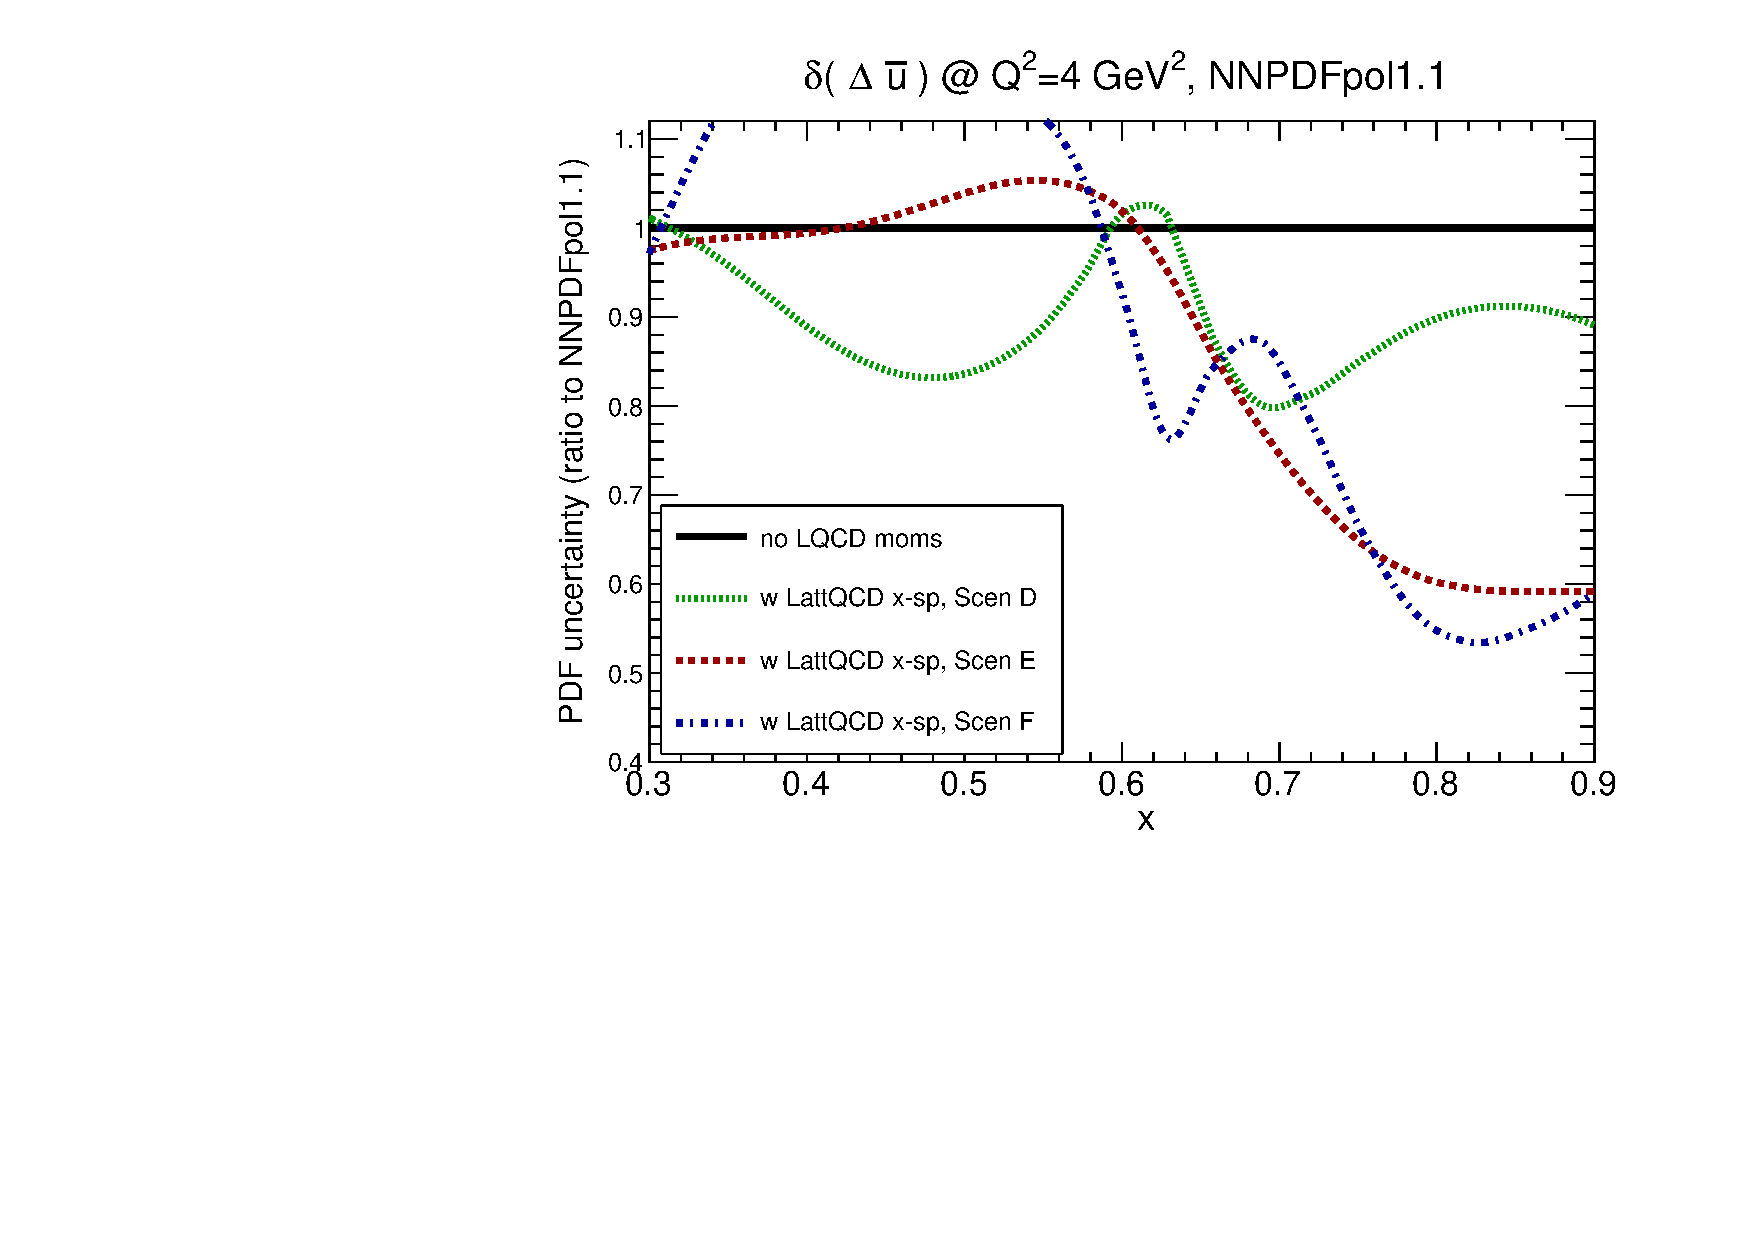
\includegraphics[scale=0.45]{plots/xubar-pol-lattice-relerr-xdata-xspace.pdf}
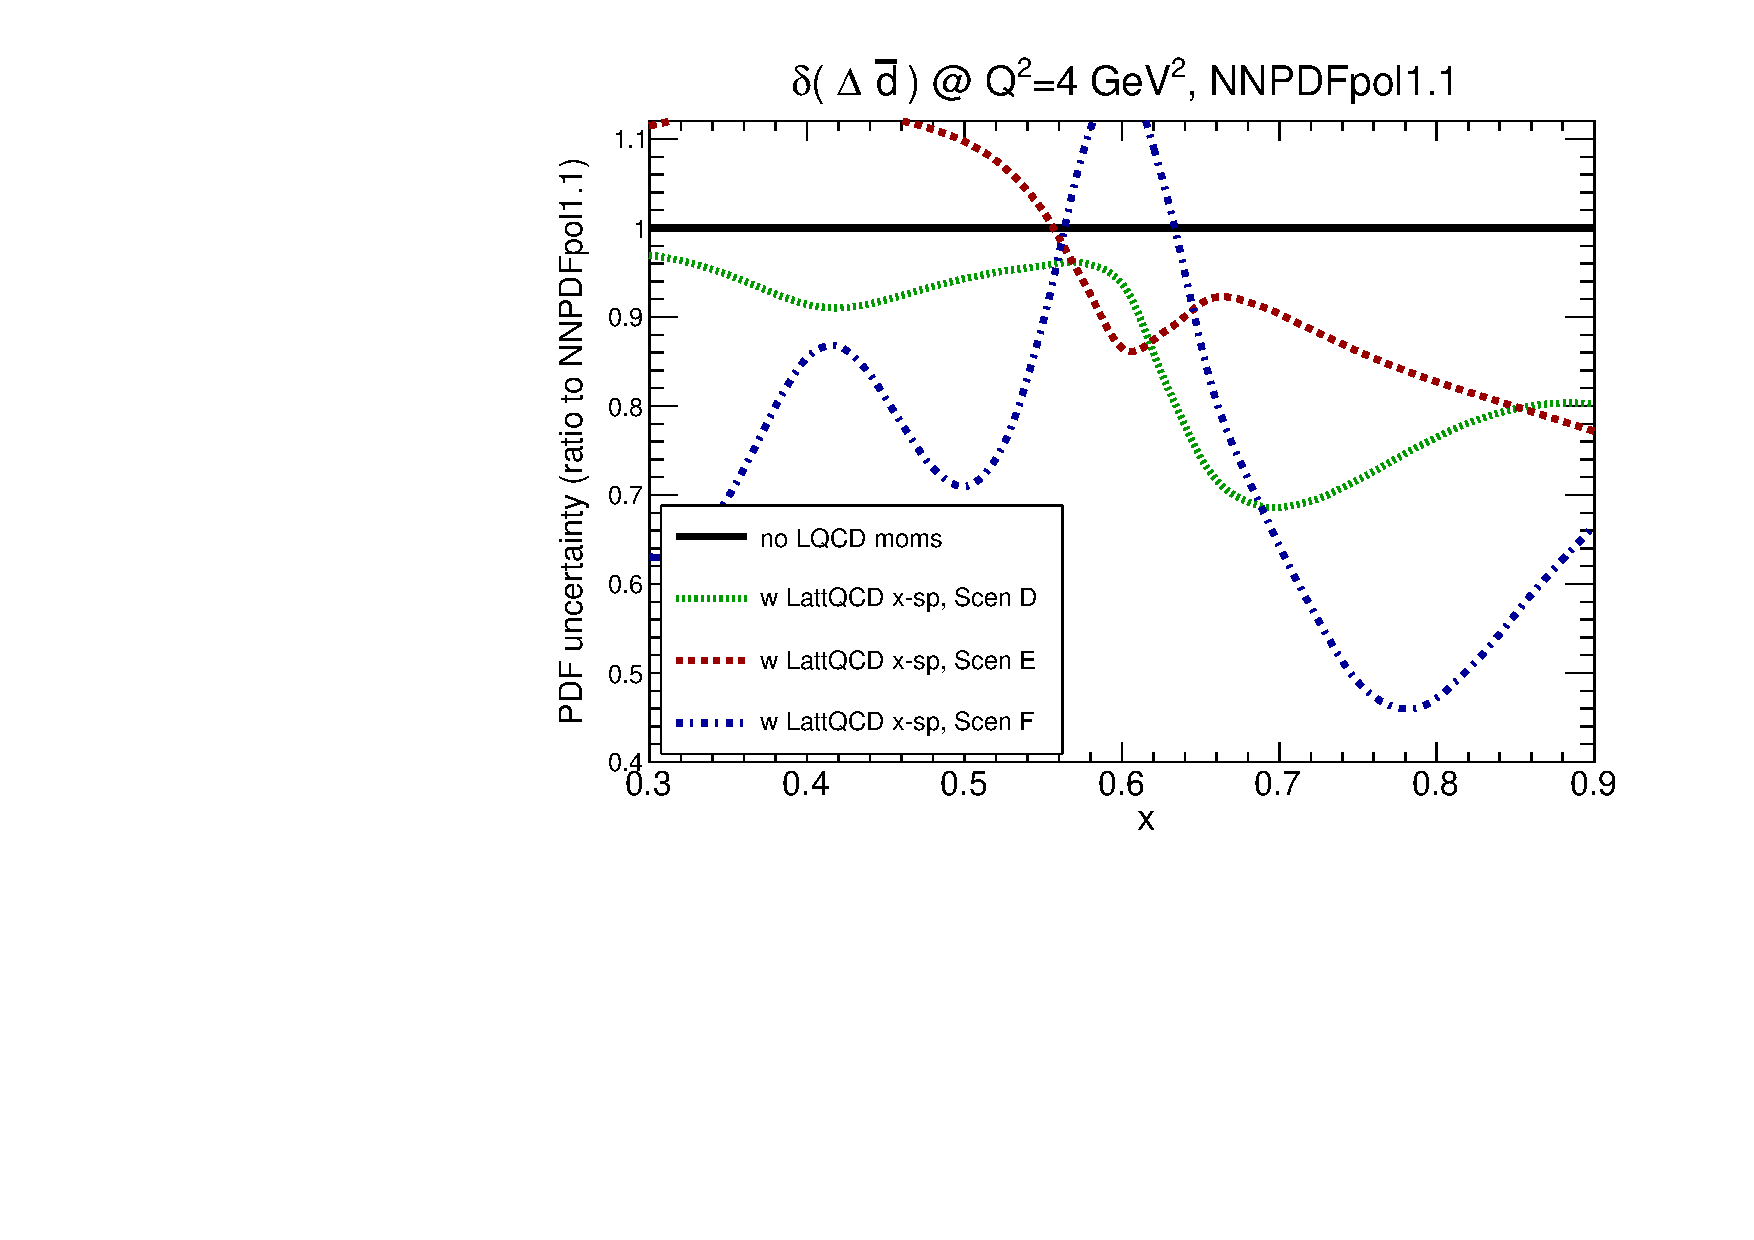
\includegraphics[scale=0.45]{plots/xdbar-pol-lattice-relerr-xdata-xspace.pdf}
\caption{\small The ratio of PDF uncertainties to the original
  NNPDF3.1 (NNPDFpol1.1) in the fits where lattice-QCD pseudo-data
  on $x$-space PDFs has been added to the global unpolarized
  (polarized) analysis.
  %
  Specifically, we show the impact on the PDF uncertainties
  in $\bar{u}$ and $\bar{d}$ at large-$x$ in the upper
  plots, with the corresponding comparison for $\Delta\bar{u}$
  and $\Delta\bar{d}$ in the lower plots.
}    
\label{fig:impactxspace}
\end{figure}
%---------------------------------------------------------------------

Specifically, from Fig.~\ref{fig:impactxspace} we find that
in unpolarized case the large-$x$ PDF uncertainties can be reduced
down to $60\%$ of its original value.
%
We also find that there are no large
differences between the three
scenarios, suggesting that a direct lattice-QCD calculation
of $x u-x d$ does not need to reach uncertainties
at the few-percent level in order to impact positively
the PDFs.
%
In the polarized case, we find a similar result but the reduction
of PDF uncertainties can be more marked.
%
For instance in the case of $\Delta \bar{d}$, at $x\simeq 0.8$
the resulting PDF uncertainty from scenario C is less than 50\%
of the original one.

Then in Table~\ref{tab:neffxspace} we indicate the effective number of replicas
$N_{\rm eff}$, Eq.~(\ref{eq:effnrep}), remaining when
the pseudo-data
    on the lattice-QCD calculations
    of Eqns.~(\ref{eq:isotriplet_unpol})
and~(\ref{eq:isotriplet_pol}).
   is included in the global
   unpolarized and polarized fits.
   %
   Also here we find a marked decrease of $N_{\rm rep}$
   for the three scenarios considered,
   in particular for the unpolarized case.
   %
   For example, in the most optimistic scenario F, only
   64 effective replicas remain out of the
   original sample of $N_{\rm rep}=1000$ replicas.
   %
   See Table~\ref{tab:neff} for the corresponding
   information at the level of PDF moments.
   
%%%%%%%%%%%%%%%%%%%%%%%%%%%%%%%%%%%%%%%%%%%%%%
\begin{table}[h!]
  \centering
  \renewcommand{\arraystretch}{1.3} 
  \begin{tabular}{c|c|c}
    \hline
    &  NNPDF3.1  &  NNPDFpol1.1 \\
    \hline
    \hline
    $N_{\rm rep}$ original   &   1000 &  100   \\
    \hline
     $N_{\rm eff}$ Scenario D    &   376  &  41   \\
     $N_{\rm eff}$ Scenario E    &   173   &   35  \\
     $N_{\rm eff}$ Scenario F   &   64  &   22  \\
    \hline
  \end{tabular}
  \caption{\small The effective number of replicas
    $N_{\rm eff}$, Eq.~(\ref{eq:effnrep}), remaining when the pseudo-data
    on the lattice-QCD calculations
    of Eqns.~(\ref{eq:isotriplet_unpol})
and~(\ref{eq:isotriplet_pol}).
   is included in the global
    unpolarized and polarized fits. 
    \label{tab:neffxspace}
  }
\end{table}
%%%%%%%%%%%%%%%%%%%%%%%%%%%%%%%%%%%%%%%%%%%%%%

We emphasize that
the results of this exercise have to be interpreted
with some care.
%
First of all, the results depend sensitively on the specific values of
$\left\{ x_i \right\}$
that we have assumed for the lattice-QCD calculation,
as well as on the values
of the associated uncertainties $\delta_L$.
%
Also, the quantitative results would vary if a different input PDF set
was used, for example the HERAPDF2.0 set that was used for
the Hessian profiling exercise of Sect.~\ref{sec:hessianprofiling}.
%
But even accounting for these caveats, is clear that a direct
computation of the isotriplet combination $x u-x d$ on the lattice
has the potential to constrain the large-$x$ PDFs in
a more significant way that the corresponding PDF moments calculation,
specially in the unpolarized case.
%
And given the importance of large-$x$ antiquarks for LHC phenomenology,
pursuing these calculations should be high on the list
of priorities of the lattice-QCD community.

%%%%%%%%%%%%%%%%%%%%%%%%%%%%%%%%%%%%%%%%%%%%%%%%%
